\documentclass{article}
\PassOptionsToPackage{numbers, compress}{natbib}
\usepackage[preprint]{neurips_2025}
\usepackage[utf8]{inputenc}
\usepackage[T1]{fontenc}
\usepackage{hyperref}
\usepackage{url}
\usepackage{booktabs}
\usepackage{multirow}
\usepackage{amsfonts}
\usepackage{amsmath}
\usepackage{nicefrac}
\usepackage{microtype}
\usepackage[table]{xcolor}
\usepackage{graphicx}
\usepackage{caption}
\captionsetup{font=small, skip=3pt}
\setlength{\textfloatsep}{8pt plus 2pt minus 2pt}
\setlength{\abovedisplayskip}{4pt}\setlength{\belowdisplayskip}{4pt}

\newcommand{\nmse}{\mathrm{nMSE}}
\newcommand{\LS}{\mathrm{LS}}

\title{One Prior for Many Graph Inverse Problems?\\
\large A Controlled Study of Operator and Dataset Transfer for Learned Graph Regularisers}

\author{%
  Yakov Gelerenter \\
  \texttt{ygelerenter8876@gmail.com} \\
  \And
  Yoav Lavi \\
  \texttt{laviyoav@post.bgu.ac.il} \\
}

\begin{document}
\maketitle

\begin{abstract}
GRIP learns one regulariser per graph inverse problem. We ask whether a \emph{single} learned prior can serve
several graph inverse problems and how far it transfers. One unrolled variational GNN solver (101k parameters,
built on the official GRIP code) is trained on a mixture of forward operators over a fixed signal family and
tested (A) on a fifth operator it never saw, signals held fixed, and (B) on datasets and graphs it never saw,
all operators known; the tasks are denoising, inpainting, sensor recovery, source localization and PDE-state
reconstruction. Against validation-tuned Tikhonov and graph-Laplacian solvers, an
early-stopped least-squares solver and the same network trained from scratch on the target task, the
shared prior reaches similar mean performance to from-scratch training on the two tasks whose measurements leave a null
space (inpainting, sensor recovery), where it is also the only method that improves on zero-fill. On denoising
a tuned scalar shrinkage beats every learned model, and on the two ill-conditioned operators (source
localization, PDE) every learned model, including the one trained from scratch, is clearly worse than plain
conjugate gradients. A test-time ablation shows that neither the CG budget nor the learned data-consistency
weight explains the gap: with both removed every learned model reaches 0.47 nMSE on source localization
against 0.17 for plain CG at the same budget, because each unrolled iteration restarts the data solve at the
prior's output. Dataset transfer is mostly negative: the prior beats the tuned classical solvers only on
inpainting of three of five held-out datasets, and a tuned graph-Laplacian solver wins sensor recovery. Learned models are reported over three training seeds; protocol, code and
checkpoints are released.
\end{abstract}

\section{Introduction and research question}
A graph inverse problem recovers a node signal $x \in \mathbb{R}^{n}$ on a graph from a measurement
$b = A x + \epsilon$, where the forward operator $A$ encodes the physics of the measurement and $\epsilon$ is
noise. Different operators define the classical tasks of graph signal recovery \citep{ortega2018gsp}: identity
(denoising), node masks (inpainting, sensor recovery), diffusion (source localization) and the heat kernel
(PDE-state reconstruction). Because $A$ is rank deficient or ill conditioned, a prior on $x$ is required. GRIP
\citep{eliasof2025grip} learns it with a graph network inside an unrolled solver, \emph{one network per operator}.

We ask the foundation-model question for this setting: \textbf{can one learned prior serve many graph inverse
problems, and does it transfer to problems it was not trained on?} Following the advice of the GRIP authors,
we isolate the two possible shifts. In experiment~A the signal family is fixed (weekly chickenpox counts on the
20-county Hungarian graph, CPOX) and only the operator changes: the model trains on four operators and is
tested on the fifth. In experiment~B all five operators are known and the dataset (hence the graph, its size,
and the signal statistics) is held out. Our contributions are:
(i) a leave-one-operator-out and a leave-one-dataset-out protocol for graph inverse problems with fixed
splits, validation-based model selection and three seeds;
(ii) a comparison of the shared prior against four baselines, two of them tuned classical regularisers and one
the same network trained from scratch at equal budget; and
(iii) a mostly negative result with a diagnosis: in our setting the shared prior transfers across operators only
where the data term is uninformative (null spaces); no learned model in our budget beats plain conjugate
gradients on the ill-conditioned operators, and a test-time ablation attributes the gap to the unrolled scheme
(the data solve restarts at the prior's output every iteration), not to the solver depth or the weight.

\paragraph{Related work.}
Learned regularisation for inverse problems ranges from unrolled optimisation \citep{gregor2010lista,
monga2021unrolling} and plug-and-play priors \citep{venkatakrishnan2013pnp} to data-driven methods at large
\citep{arridge2019datadriven}; GRIP \citep{eliasof2025grip} brings unrolled variational solvers to graphs, and
our model is its solver with a shared backbone and task heads. Tikhonov regularisation and early-stopped
iterations are the classical references \citep{hansen1998rank, engl1996regularization} and our baselines.
Foundation models \citep{bommasani2021foundation} for inverse problems exist in imaging, where one network is
trained across many operators \citep{terris2025ram}; we ask the analogous question on graphs at small scale
with controlled shifts, on PyTorch Geometric Temporal datasets \citep{rozemberczki2021pgt}.

\section{Setup and method}
\paragraph{Tasks.} All tasks share the target $x$, the node signal of one graph snapshot, and differ in $A$
(Table~\ref{tab:tasks} in the appendix): \emph{denoising}, $A = I$ with Gaussian noise $\sigma = 0.25$, the only
noisy task; \emph{inpainting}, a random mask keeping 6 of the nodes; \emph{sensor recovery}, one BFS-grown patch
of 5 sensors; \emph{source localization}, $A = \hat A^{4}$ (four diffusion steps, condition number
$\kappa \approx 7 \cdot 10^{5}$ on CPOX); \emph{PDE-state reconstruction}, $A = \exp(-20 L)$
($\kappa \approx 4 \cdot 10^{9}$). Masks and patches are resampled every batch. Graphs are made undirected and
GCN-normalised \citep{kipf2017gcn}; $\hat A$ is the normalised adjacency, $L = I - \hat A$ the normalised
Laplacian. The two mask tasks have a null space; the two diffusion tasks are invertible but ill conditioned.


\paragraph{Model.} We use GRIP's unrolled solver with three changes. A \emph{shared backbone} $R_\theta$ (a 32-layer, 32-channel hyperbolic graph ResNet, the learned prior) maps a
latent state to a reference signal; a \emph{task encoder/head pair} (two linear layers, $< 1\,\%$ of the
parameters) maps the measurement and the observation mask into the latent space and back; and a
\emph{data-consistency step} per unrolled iteration solves
\begin{equation}
  x^{(k+1)} = \arg\min_x \; \|A x - b\|^{2} + \lambda_{\text{task}} \|x - R_\theta(x^{(k)})\|^{2}
  \label{eq:prox}
\end{equation}
with 5 conjugate-gradient (CG) steps warm-started at the backbone's output, $\lambda_{\text{task}}$ learned
(closed form for denoising); 5 unrolled iterations, 101k parameters in total. Before a task head exists, a
shared encoder/head is used, which gives the \emph{zero-shot} model for an unseen task.

\paragraph{Training protocol.} Three phases per run. (1) \emph{Backbone}, 40 epochs: backbone and shared
head on the training tasks, one task per epoch in rotation, loss
$\tfrac12\,[\nmse(\hat x, x) + \nmse(A \hat x, A x)]$, $\nmse(\hat x, x) = \|\hat x - x\|^{2} / \|x\|^{2}$.
(2) \emph{Heads}, 16 epochs: backbone frozen, task heads on the training tasks.
(3) \emph{Adaptation}, 4 epochs: backbone frozen, the held-out task's head on the full CPOX training split
(A only; in B the held-out dataset is never trained on and phase 3 is 4 more head epochs on the training
datasets). Phase 1 yields the zero-shot checkpoint, phase 3 the task-head checkpoint. Adam, lr $10^{-3}$
($10^{-4}$ for heads), batches of 4 snapshots, gradient clipping at 1. Every phase selects its checkpoint on a
\emph{validation split} (last 10\,\% of the CPOX training weeks; the chronological tail of each training
dataset in B); the test split is evaluated once per phase.

\paragraph{Baselines.} The course brief asks for meaningful baselines; ours are
(a) $x = b$, the measurement itself, and $x = 0$ ($\nmse = 1$);
(b) \emph{least squares}: 25 CGLS steps from zero with no prior, which on the ill-conditioned operators is an
early-stopped, hence implicitly regularised, solution \citep{hansen1998rank};
(c) \emph{Tikhonov} $\arg\min_x \|Ax - b\|^{2} + \lambda \|x\|^{2}$ and
(d) \emph{graph-Laplacian} $\arg\min_x \|Ax - b\|^{2} + \lambda\, x^{\top} L x$, solved by CG on the normal
equations, with $(\lambda, \text{CG steps}) \in \{0, 10^{-6}, \dots, 10^{2}\} \times \{5, 25, 100\}$
chosen per task on the same validation split the learned models were selected on;
(e) the \emph{same network trained from scratch} on the target task alone for 60 epochs, the budget of a
full foundation run (phases 1--3): our ablation of pretraining, which removes the multi-task backbone only.

\paragraph{Evaluation protocol.} Metric: nMSE on the test split, averaged over batches of 4 snapshots
(lower is better; 1 means predicting zero). Within a table every row inverts \emph{identical} measurements
(same masks, sensors and noise draws, seeded on the CPU generator, hence device independent). Splits: CPOX
test = the last 10\,\% of weeks; in B the whole held-out dataset is the test set (Windmill 5\,\% and
WikiMaths 20\,\% of their snapshots; both are test-only). In B every dataset is z-normalised with its own
target mean and standard deviation, the held-out one included, so B is an \emph{oracle-normalised} benchmark.
Learned rows report mean $\pm$ sample standard deviation over three training seeds (0--2); the classical rows
are deterministic on the same measurements and have no spread.

\section{Experiments}
\paragraph{A: transfer to an unseen operator (CPOX).}
Table~\ref{tab:a} reports, for every task, the model that had \emph{that} task held out (the diagonal of the
full $5 \times 5$ table in Appendix~\ref{app:full}) against the baselines. Three observations.
\emph{Null-space tasks.} For inpainting and sensor recovery no classical solver beats zero-fill (the tuned
$\lambda$ is $\approx 0$), and the learned prior is the only thing that does. The pretrained model transfers: zero-shot
sensor recovery ties the network trained from scratch on that task (0.732 vs.\ 0.733) and the adapted head is
ahead (0.725); zero-shot inpainting stays at zero-fill (0.683) and the adapted head recovers most of the gap
to from-scratch (0.668 vs.\ 0.658). Gains over zero-fill are only 0.02--0.04 nMSE.
\emph{Denoising.} A validation-tuned scalar shrinkage ($x = b / 1.32$) reaches 0.281 and beats every learned
model, from scratch (0.313) and pretrained (0.301--0.317); the best learned denoising cells of the full table
(0.278) only tie it: the prior adds nothing beyond shrinkage on this heavy-tailed count signal.
\emph{Ill-conditioned operators.} Every learned model is far behind 25 plain CGLS steps: source localization
0.61--0.65 vs.\ 0.42, PDE 0.73--0.80 vs.\ 0.61. The tuned classical solvers select $\lambda \le 10^{-6}$, so
the CG budget is the regulariser; they match least squares on source localization (0.428), and on PDE the
validation split prefers 100 steps where the test split prefers 25 (0.714 vs.\ 0.613), a validation/test
shift we report as is. The pretrained models are a further 0.03--0.07 behind from-scratch here. Seed spread
is small everywhere (std $\le 0.02$).

\begin{table}[t]
\centering\footnotesize\setlength{\tabcolsep}{4pt}
\begin{tabular}{lccccc}
\toprule
CPOX test weeks, nMSE $\downarrow$ & denoise & inpaint & sensor & source-loc & PDE \\
\midrule
$x = b$ (measurement) & 0.383 & 0.687 & 0.758 & 0.742 & 0.817 \\
least squares, 25 CGLS steps & 0.383 & 0.687 & 0.758 & \textbf{0.421} & \textbf{0.613} \\
Tikhonov LS, tuned & \textbf{0.281} & 0.687 & 0.758 & 0.428 & 0.714 \\
graph-Laplacian LS, tuned & 0.302 & 0.687 & 0.758 & 0.428 & 0.713 \\
single-task net from scratch (60 ep.) & 0.312{\scriptsize$\pm$0.012} & \textbf{0.658}{\scriptsize$\pm$0.011} & 0.733{\scriptsize$\pm$0.007} & 0.609{\scriptsize$\pm$0.007} & 0.730{\scriptsize$\pm$0.006} \\
\midrule
pretrained, held out, zero-shot & 0.317{\scriptsize$\pm$0.018} & 0.683{\scriptsize$\pm$0.020} & 0.732{\scriptsize$\pm$0.006} & 0.652{\scriptsize$\pm$0.001} & 0.805{\scriptsize$\pm$0.001} \\
pretrained, held out, + task head & 0.301{\scriptsize$\pm$0.005} & 0.668{\scriptsize$\pm$0.005} & \textbf{0.725}{\scriptsize$\pm$0.005} & 0.639{\scriptsize$\pm$0.003} & 0.804{\scriptsize$\pm$0.001} \\
\bottomrule
\end{tabular}

\caption{Experiment A. CPOX test nMSE (mean $\pm$ std, 3 seeds) of the model with the column's task held out,
against the baselines; best per column in bold. Tuned classical rows use the validation-optimal $(\lambda, \text{CG steps})$.}
\label{tab:a}
\end{table}

\paragraph{B: transfer to an unseen dataset.}
Table~\ref{tab:b} compares, per held-out dataset, the best tuned classical solver with the pretrained model
(task heads trained on the training datasets, zero-shot on the held-out one; the shared-head model is within
0.02, Table~\ref{tab:b_full}). The outcome is mostly negative and follows the graphs. On the two complete
graphs (PedalMe, Windmill) the Laplacian has two eigenvalues, so the two diffusion tasks reduce to recovering
the mean and all methods coincide; there the prior wins inpainting (0.49 vs.\ 0.55, 0.89 vs.\ 0.98) but loses
sensor recovery to the tuned graph-Laplacian solver (0.60 vs.\ 0.58, 0.91 vs.\ 0.83), whose smoothness penalty
is what a clustered sensor patch needs. On the sparse 675-node Montevideo graph the model is behind the tuned
solvers on every task (source localization 0.45 vs.\ 0.27); on WikiMaths it leads only on inpainting, by 0.01.
CPOX held out is the worst case: trained on PedalMe (15 nodes) and Montevideo only, the model is worse than
least squares on four of five tasks with a seed spread up to 0.23. A prior trained on two or three small
spatio-temporal graphs does not carry over to a graph with different degree statistics; what transfers is the
inpainting behaviour, and a tuned Laplacian prior matches it on sensor recovery.

\begin{table}[t]
\centering\footnotesize\setlength{\tabcolsep}{4pt}
\begin{tabular}{lccccc}
\toprule
held-out dataset & denoise & inpaint & sensor & source-loc & PDE \\
\midrule
CPOX (20 nodes) & 0.400 (0.400) & 0.812 (0.694) & 0.789 (0.757) & 0.805 (0.384) & 0.726 (0.563) \\
Montevideo (675) & 0.146 (0.120) & 1.023 (0.991) & 1.050 (0.992) & 0.446 (0.269) & 0.611 (0.528) \\
PedalMe (15, complete) & 0.116 (0.090) & \textbf{0.493} (0.545) & 0.603 (0.575) & 0.706 (0.706) & 0.706 (0.706) \\
WikiMaths (1068) & 0.075 (0.061) & \textbf{0.986} (0.995) & 0.986 (0.991) & 0.575 (0.471) & 0.586 (0.552) \\
Windmill (319, complete) & 0.094 (0.085) & \textbf{0.890} (0.981) & 0.908 (0.830) & 0.354 (0.354) & 0.354 (0.354) \\
\bottomrule
\end{tabular}

\caption{Experiment B. Zero-shot nMSE on the held-out dataset, mean of 3 seeds: the pretrained model with task
heads, and in parentheses the best classical solver (plain, tuned Tikhonov or tuned graph-Laplacian least
squares); bold where the pretrained model is lower by at least 0.005. All rows (incl.\ the shared-head model)
and stds in Table~\ref{tab:b_full}.}
\label{tab:b}
\end{table}

\section{Ablation, limitations and conclusion}
\paragraph{Ablation: is the solver the bottleneck?}
The learned models run 5 CG steps per unrolled iteration, 25 in total, the budget of the least-squares row they
lose to, but warm-started at the prior and pulled towards it by $\lambda_{\text{task}}$ (eq.~\ref{eq:prox}).
We re-evaluate the \emph{same} checkpoints with the data-consistency step changed at test time: 1, 5 or 25 CG
steps per iteration, 10 instead of 5 unrolled iterations, and $\lambda_{\text{task}}$ overridden to $10^{-8}$
(a pure least-squares step from the prior's output), against least squares at 5, 25 and 100 CGLS steps
(Table~\ref{tab:abl}; all tasks, seeds and zero-shot rows in Appendix~\ref{app:full}). Source localization is
noise free, so plain CG keeps improving with budget (0.63, 0.42, 0.17); the learned models do not follow.
Budget alone (25 CG steps per iteration, 125 in total) takes the from-scratch network from 0.61 to 0.51 and
the pretrained one from 0.64 to 0.63. Weight alone leaves the from-scratch model unchanged (its learned weight
is already $10^{-4}$--$10^{-5}$), moves the pretrained one from 0.64 to 0.63, and lifts the pretrained PDE
model from 0.80 to 0.73: the untrained $\lambda = 0.01$ of a held-out task does anchor that iterate. Both
together land every learned model at 0.47 on source localization and 0.72 on PDE, the error of a 25-step CG
run from zero (0.42, 0.61) and far from plain CG at the same budget (0.17, 0.61). The reason is
eq.~\ref{eq:prox}: every unrolled iteration restarts CG at $R_\theta(x^{(k)})$, no better a starting point
than zero on these operators, so the solver never accumulates more than one iteration's progress. With a
single CG step all models collapse to the $x = b$ level (0.78--0.79): the data-consistency step, not the
prior, does the work. Doubling the unrolled depth changes nothing; the mask tasks are unaffected by every setting.

\begin{table}[t]
\centering\footnotesize
\begin{tabular}{llccc}
\toprule
model & test-time solver & inpaint & source-loc & PDE \\
\midrule
\multirow{3}{*}{least squares (CGLS)} & 25 steps & 0.687 & 0.421 & 0.613 \\
 & 5 steps & 0.687 & 0.632 & 0.716 \\
 & 100 steps & 0.687 & 0.173 & 0.610 \\
\midrule
\multirow{5}{*}{from scratch} & as trained ($5 \times 5$) & 0.658 & 0.608 & 0.729 \\
 & 1 CG step / it. & 0.658 & 0.778 & 0.829 \\
 & 25 CG steps / it. & 0.658 & 0.514 & 0.724 \\
 & $\lambda = 10^{-8}$ & 0.658 & 0.609 & 0.729 \\
 & $\lambda = 10^{-8}$, 25 CG/it. & 0.658 & 0.471 & 0.722 \\
\midrule
\multirow{5}{*}{pretrained, + task head} & as trained ($5 \times 5$) & 0.668 & 0.639 & 0.804 \\
 & 1 CG step / it. & 0.668 & 0.784 & 0.830 \\
 & 25 CG steps / it. & 0.668 & 0.627 & 0.804 \\
 & $\lambda = 10^{-8}$ & 0.668 & 0.627 & 0.728 \\
 & $\lambda = 10^{-8}$, 25 CG/it. & 0.668 & 0.471 & 0.717 \\
\bottomrule
\end{tabular}

\caption{Test-time solver ablation: the checkpoints of Table~\ref{tab:a} re-run with a different data-consistency
step, no retraining (held-out-task cells, mean of 3 seeds; zero-shot and 10-iteration rows, all tasks and stds in
Table~\ref{tab:abl_full}).}
\label{tab:abl}
\end{table}

\paragraph{Limitations.} (1) Scale: one signal family in A (CPOX, 520 weekly snapshots of a 20-node graph),
small spatio-temporal graphs in B, one 101k-parameter architecture (the brief), no architecture sweep. (2) Head
adaptation is supervised on the full training split; no few-shot claim. (3) B is oracle-normalised; its training
mixes are two or three datasets, two of them complete graphs on which two operators are trivial. (4) nMSE is
averaged per batch, up-weighting low-energy snapshots. (5) The classical grid has a 100-step CG ceiling.

\paragraph{Conclusion.} A single learned graph prior does transfer across forward operators, but only where
the measurement leaves a null space; there it matches a network trained from scratch at equal budget and is the
only method that improves on the tuned classical solvers. On denoising a tuned scalar shrinkage is as good as
any learned model. On the ill-conditioned operators neither the shared prior nor a dedicated network beats
plain conjugate gradients, and the ablation shows why: not the CG budget or the weight, but the restart of the
data solve at the prior's output in every unrolled iteration. Across datasets the prior wins only inpainting.
``One prior for many graph inverse problems'' thus holds for the null-space tasks and not yet for the
ill-conditioned ones; an unrolled scheme that keeps the CG state across iterations and uses the prior only as a
penalty is the natural next experiment.

\clearpage
\bibliographystyle{plainnat}
\begin{thebibliography}{15}

\bibitem[Arridge et~al.(2019)]{arridge2019datadriven}
S.~Arridge, P.~Maass, O.~\"Oktem, and C.-B. Sch\"onlieb.
\newblock Solving inverse problems using data-driven models.
\newblock \emph{Acta Numerica}, 28:1--174, 2019.

\bibitem[Bommasani et~al.(2021)]{bommasani2021foundation}
R.~Bommasani et~al.
\newblock On the opportunities and risks of foundation models.
\newblock \emph{arXiv:2108.07258}, 2021.

\bibitem[Eliasof et~al.(2025)]{eliasof2025grip}
M.~Eliasof, M.~S.~R. Siddiqui, C.-B. Sch\"onlieb, and E.~Haber.
\newblock Learning regularization for graph inverse problems.
\newblock In \emph{AAAI Conference on Artificial Intelligence}, 39(16):16471--16479, 2025.

\bibitem[Engl et~al.(1996)]{engl1996regularization}
H.~W. Engl, M.~Hanke, and A.~Neubauer.
\newblock \emph{Regularization of Inverse Problems}.
\newblock Kluwer, 1996.

\bibitem[Gregor and LeCun(2010)]{gregor2010lista}
K.~Gregor and Y.~LeCun.
\newblock Learning fast approximations of sparse coding.
\newblock In \emph{International Conference on Machine Learning}, 2010.

\bibitem[Hansen(1998)]{hansen1998rank}
P.~C. Hansen.
\newblock \emph{Rank-Deficient and Discrete Ill-Posed Problems}.
\newblock SIAM, 1998.

\bibitem[Kipf and Welling(2017)]{kipf2017gcn}
T.~N. Kipf and M.~Welling.
\newblock Semi-supervised classification with graph convolutional networks.
\newblock In \emph{International Conference on Learning Representations}, 2017.

\bibitem[Monga et~al.(2021)]{monga2021unrolling}
V.~Monga, Y.~Li, and Y.~C. Eldar.
\newblock Algorithm unrolling: Interpretable, efficient deep learning for signal and image processing.
\newblock \emph{IEEE Signal Processing Magazine}, 38(2):18--44, 2021.

\bibitem[Ortega et~al.(2018)]{ortega2018gsp}
A.~Ortega, P.~Frossard, J.~Kova\v{c}evi\'c, J.~M.~F. Moura, and P.~Vandergheynst.
\newblock Graph signal processing: Overview, challenges, and applications.
\newblock \emph{Proceedings of the IEEE}, 106(5):808--828, 2018.

\bibitem[Rozemberczki et~al.(2021)]{rozemberczki2021pgt}
B.~Rozemberczki et~al.
\newblock PyTorch Geometric Temporal: Spatiotemporal signal processing with neural machine learning models.
\newblock In \emph{ACM International Conference on Information and Knowledge Management}, 2021.

\bibitem[Terris et~al.(2025)]{terris2025ram}
M.~Terris, S.~Hurault, M.~Song, and J.~Tachella.
\newblock Reconstruct anything model: a lightweight foundation model for computational imaging.
\newblock \emph{arXiv:2503.08915}, 2025.

\bibitem[Venkatakrishnan et~al.(2013)]{venkatakrishnan2013pnp}
S.~V. Venkatakrishnan, C.~A. Bouman, and B.~Wohlberg.
\newblock Plug-and-play priors for model based reconstruction.
\newblock In \emph{IEEE Global Conference on Signal and Information Processing}, 2013.

\end{thebibliography}

\clearpage
\appendix
\section{Full result tables}
\label{app:full}
Tables~\ref{tab:a_full}--\ref{tab:abl_full} are the complete evaluator outputs (\texttt{results/*/*.csv}).
In Table~\ref{tab:a_full} the shaded cell of each model row is its held-out task (the transfer number); the
other cells are tasks that row trained on. The raw tables as rendered by the evaluation scripts are the
\texttt{.png} files next to those CSVs.

\begin{table}[h]
\centering\scriptsize
\begin{tabular}{lccccc}
\toprule
CPOX test weeks, nMSE $\downarrow$ & denoise & inpaint & sensor & source-loc & PDE \\
\midrule
$x = b$ (measurement) & 0.383 & 0.687 & 0.758 & 0.742 & 0.817 \\
least squares, 25 CGLS steps & 0.383 & 0.687 & 0.758 & \textbf{0.421} & \textbf{0.613} \\
Tikhonov LS, tuned & \textbf{0.281} & 0.687 & 0.758 & 0.428 & 0.714 \\
graph-Laplacian LS, tuned & 0.302 & 0.687 & 0.758 & 0.428 & 0.713 \\
single-task net from scratch (60 ep.) & 0.312{\scriptsize$\pm$0.012} & \textbf{0.658}{\scriptsize$\pm$0.011} & 0.733{\scriptsize$\pm$0.007} & 0.609{\scriptsize$\pm$0.007} & 0.730{\scriptsize$\pm$0.006} \\
\midrule
pretrained, held out, zero-shot & 0.317{\scriptsize$\pm$0.018} & 0.683{\scriptsize$\pm$0.020} & 0.732{\scriptsize$\pm$0.006} & 0.652{\scriptsize$\pm$0.001} & 0.805{\scriptsize$\pm$0.001} \\
pretrained, held out, + task head & 0.301{\scriptsize$\pm$0.005} & 0.668{\scriptsize$\pm$0.005} & \textbf{0.725}{\scriptsize$\pm$0.005} & 0.639{\scriptsize$\pm$0.003} & 0.804{\scriptsize$\pm$0.001} \\
\midrule
denoise held out, zero-shot & \cellcolor{blue!10}0.317{\scriptsize$\pm$0.018} & 0.654{\scriptsize$\pm$0.004} & 0.720{\scriptsize$\pm$0.005} & 0.634{\scriptsize$\pm$0.003} & 0.729{\scriptsize$\pm$0.000} \\
inpaint held out, zero-shot & 0.296{\scriptsize$\pm$0.014} & \cellcolor{blue!10}0.683{\scriptsize$\pm$0.020} & 0.750{\scriptsize$\pm$0.022} & 0.615{\scriptsize$\pm$0.014} & 0.726{\scriptsize$\pm$0.003} \\
sensor held out, zero-shot & 0.292{\scriptsize$\pm$0.011} & 0.662{\scriptsize$\pm$0.007} & \cellcolor{blue!10}0.732{\scriptsize$\pm$0.006} & 0.628{\scriptsize$\pm$0.007} & 0.729{\scriptsize$\pm$0.002} \\
source-loc held out, zero-shot & 0.284{\scriptsize$\pm$0.011} & 0.673{\scriptsize$\pm$0.023} & 0.732{\scriptsize$\pm$0.029} & \cellcolor{blue!10}0.652{\scriptsize$\pm$0.001} & 0.731{\scriptsize$\pm$0.001} \\
PDE held out, zero-shot & 0.283{\scriptsize$\pm$0.007} & 0.675{\scriptsize$\pm$0.015} & 0.734{\scriptsize$\pm$0.031} & 0.633{\scriptsize$\pm$0.001} & \cellcolor{blue!10}0.805{\scriptsize$\pm$0.001} \\
denoise held out, + task heads & \cellcolor{blue!10}0.301{\scriptsize$\pm$0.005} & 0.653{\scriptsize$\pm$0.002} & 0.717{\scriptsize$\pm$0.003} & 0.632{\scriptsize$\pm$0.002} & 0.727{\scriptsize$\pm$0.002} \\
inpaint held out, + task heads & 0.297{\scriptsize$\pm$0.015} & \cellcolor{blue!10}0.668{\scriptsize$\pm$0.005} & 0.739{\scriptsize$\pm$0.012} & 0.611{\scriptsize$\pm$0.015} & 0.725{\scriptsize$\pm$0.003} \\
sensor held out, + task heads & 0.292{\scriptsize$\pm$0.014} & 0.655{\scriptsize$\pm$0.002} & \cellcolor{blue!10}0.725{\scriptsize$\pm$0.005} & 0.621{\scriptsize$\pm$0.011} & 0.727{\scriptsize$\pm$0.002} \\
source-loc held out, + task heads & 0.278{\scriptsize$\pm$0.000} & 0.657{\scriptsize$\pm$0.004} & 0.718{\scriptsize$\pm$0.005} & \cellcolor{blue!10}0.639{\scriptsize$\pm$0.003} & 0.729{\scriptsize$\pm$0.000} \\
PDE held out, + task heads & 0.280{\scriptsize$\pm$0.002} & 0.659{\scriptsize$\pm$0.006} & 0.718{\scriptsize$\pm$0.003} & 0.630{\scriptsize$\pm$0.001} & \cellcolor{blue!10}0.804{\scriptsize$\pm$0.001} \\
\bottomrule
\end{tabular}

\caption{Experiment A, full table (CPOX test weeks, nMSE, mean $\pm$ std over 3 seeds).}
\label{tab:a_full}
\end{table}

\begin{table}[h]
\centering\scriptsize\setlength{\tabcolsep}{2pt}
\begin{tabular}{llccccc}
\toprule
held-out dataset & method & denoise & inpaint & sensor & source-loc & PDE \\
\midrule
\multirow{5}{*}{CPOX (20 nodes)} & least squares, 25 CGLS steps & 0.474 & 0.703 & \textbf{0.757} & \textbf{0.384} & \textbf{0.563} \\
 & Tikhonov LS, tuned & 0.400 & 0.703 & \textbf{0.757} & 0.398 & 0.687 \\
 & graph-Laplacian LS, tuned & 0.413 & \textbf{0.694} & 0.888 & 0.398 & 0.687 \\
 & pretrained, shared head & 0.466{\scriptsize$\pm$0.060} & 0.831{\scriptsize$\pm$0.188} & 0.793{\scriptsize$\pm$0.052} & 0.642{\scriptsize$\pm$0.095} & 0.770{\scriptsize$\pm$0.044} \\
 & pretrained, task heads & \textbf{0.400}{\scriptsize$\pm$0.014} & 0.812{\scriptsize$\pm$0.159} & 0.789{\scriptsize$\pm$0.055} & 0.805{\scriptsize$\pm$0.228} & 0.726{\scriptsize$\pm$0.017} \\
\midrule
\multirow{5}{*}{Montevideo (675)} & least squares, 25 CGLS steps & 0.127 & \textbf{0.991} & 0.992 & 0.385 & 0.565 \\
 & Tikhonov LS, tuned & \textbf{0.120} & \textbf{0.991} & 0.992 & \textbf{0.269} & \textbf{0.528} \\
 & graph-Laplacian LS, tuned & 0.122 & 0.991 & \textbf{0.992} & \textbf{0.269} & 0.528 \\
 & pretrained, shared head & 0.148{\scriptsize$\pm$0.013} & 1.059{\scriptsize$\pm$0.055} & 1.073{\scriptsize$\pm$0.060} & 0.457{\scriptsize$\pm$0.002} & 0.612{\scriptsize$\pm$0.001} \\
 & pretrained, task heads & 0.146{\scriptsize$\pm$0.018} & 1.023{\scriptsize$\pm$0.032} & 1.050{\scriptsize$\pm$0.069} & 0.446{\scriptsize$\pm$0.009} & 0.611{\scriptsize$\pm$0.002} \\
\midrule
\multirow{5}{*}{PedalMe (15, complete)} & least squares, 25 CGLS steps & 0.102 & 0.599 & 0.710 & \textbf{0.706} & \textbf{0.706} \\
 & Tikhonov LS, tuned & 0.092 & 0.599 & 0.710 & \textbf{0.706} & \textbf{0.706} \\
 & graph-Laplacian LS, tuned & \textbf{0.090} & 0.545 & \textbf{0.575} & \textbf{0.706} & \textbf{0.706} \\
 & pretrained, shared head & 0.130{\scriptsize$\pm$0.040} & 0.499{\scriptsize$\pm$0.003} & 0.606{\scriptsize$\pm$0.007} & 0.706{\scriptsize$\pm$0.000} & 0.706{\scriptsize$\pm$0.000} \\
 & pretrained, task heads & 0.116{\scriptsize$\pm$0.038} & \textbf{0.493}{\scriptsize$\pm$0.004} & 0.603{\scriptsize$\pm$0.011} & 0.706{\scriptsize$\pm$0.000} & 0.706{\scriptsize$\pm$0.000} \\
\midrule
\multirow{5}{*}{WikiMaths (1068)} & least squares, 25 CGLS steps & 0.068 & 0.995 & 0.995 & 0.516 & 0.554 \\
 & Tikhonov LS, tuned & 0.064 & 0.995 & 0.995 & \textbf{0.471} & \textbf{0.552} \\
 & graph-Laplacian LS, tuned & \textbf{0.061} & 0.995 & 0.991 & \textbf{0.471} & 0.578 \\
 & pretrained, shared head & 0.080{\scriptsize$\pm$0.010} & 0.989{\scriptsize$\pm$0.007} & 0.988{\scriptsize$\pm$0.008} & 0.572{\scriptsize$\pm$0.036} & 0.590{\scriptsize$\pm$0.019} \\
 & pretrained, task heads & 0.075{\scriptsize$\pm$0.002} & \textbf{0.986}{\scriptsize$\pm$0.005} & \textbf{0.986}{\scriptsize$\pm$0.004} & 0.575{\scriptsize$\pm$0.017} & 0.586{\scriptsize$\pm$0.011} \\
\midrule
\multirow{5}{*}{Windmill (319, complete)} & least squares, 25 CGLS steps & 0.100 & 0.981 & 0.985 & \textbf{0.354} & 0.354 \\
 & Tikhonov LS, tuned & 0.095 & 0.981 & 0.985 & \textbf{0.354} & \textbf{0.354} \\
 & graph-Laplacian LS, tuned & \textbf{0.085} & 0.981 & \textbf{0.830} & \textbf{0.354} & 0.354 \\
 & pretrained, shared head & 0.096{\scriptsize$\pm$0.007} & \textbf{0.873}{\scriptsize$\pm$0.024} & 0.889{\scriptsize$\pm$0.021} & 0.354{\scriptsize$\pm$0.000} & 0.354{\scriptsize$\pm$0.000} \\
 & pretrained, task heads & 0.094{\scriptsize$\pm$0.008} & 0.890{\scriptsize$\pm$0.025} & 0.908{\scriptsize$\pm$0.027} & 0.354{\scriptsize$\pm$0.000} & 0.354{\scriptsize$\pm$0.000} \\
\bottomrule
\end{tabular}

\caption{Experiment B, full table (zero-shot nMSE on the held-out dataset, mean $\pm$ std over 3 seeds).}
\label{tab:b_full}
\end{table}

\begin{table}[h]
\centering\scriptsize\setlength{\tabcolsep}{3pt}
\begin{tabular}{llccccc}
\toprule
model & test-time solver & denoise & inpaint & sensor & source-loc & PDE \\
\midrule
\multirow{3}{*}{least squares (CGLS)} & 25 steps & 0.383 & 0.687 & 0.758 & 0.421 & 0.613 \\
 & 5 steps & 0.383 & 0.687 & 0.758 & 0.632 & 0.716 \\
 & 100 steps & 0.383 & 0.687 & 0.758 & 0.173 & 0.610 \\
\midrule
\multirow{6}{*}{from scratch} & as trained ($5 \times 5$) & 0.312{\scriptsize$\pm$0.012} & 0.658{\scriptsize$\pm$0.011} & 0.733{\scriptsize$\pm$0.007} & 0.608{\scriptsize$\pm$0.006} & 0.729{\scriptsize$\pm$0.005} \\
 & 1 CG step / it. & 0.312{\scriptsize$\pm$0.012} & 0.658{\scriptsize$\pm$0.011} & 0.733{\scriptsize$\pm$0.007} & 0.778{\scriptsize$\pm$0.072} & 0.829{\scriptsize$\pm$0.007} \\
 & 25 CG steps / it. & 0.312{\scriptsize$\pm$0.012} & 0.658{\scriptsize$\pm$0.011} & 0.733{\scriptsize$\pm$0.007} & 0.514{\scriptsize$\pm$0.045} & 0.724{\scriptsize$\pm$0.001} \\
 & 10 unrolled it. & 0.312{\scriptsize$\pm$0.012} & 0.657{\scriptsize$\pm$0.011} & 0.733{\scriptsize$\pm$0.007} & 0.613{\scriptsize$\pm$0.008} & 0.925{\scriptsize$\pm$0.287} \\
 & $\lambda = 10^{-8}$ & 0.312{\scriptsize$\pm$0.012} & 0.658{\scriptsize$\pm$0.011} & 0.733{\scriptsize$\pm$0.007} & 0.609{\scriptsize$\pm$0.007} & 0.729{\scriptsize$\pm$0.005} \\
 & $\lambda = 10^{-8}$, 25 CG/it. & 0.312{\scriptsize$\pm$0.012} & 0.658{\scriptsize$\pm$0.011} & 0.733{\scriptsize$\pm$0.007} & 0.471{\scriptsize$\pm$0.010} & 0.722{\scriptsize$\pm$0.003} \\
\midrule
\multirow{6}{*}{pretrained, zero-shot} & as trained ($5 \times 5$) & 0.317{\scriptsize$\pm$0.018} & 0.683{\scriptsize$\pm$0.020} & 0.732{\scriptsize$\pm$0.006} & 0.652{\scriptsize$\pm$0.001} & 0.805{\scriptsize$\pm$0.001} \\
 & 1 CG step / it. & 0.317{\scriptsize$\pm$0.018} & 0.683{\scriptsize$\pm$0.020} & 0.732{\scriptsize$\pm$0.006} & 0.790{\scriptsize$\pm$0.001} & 0.830{\scriptsize$\pm$0.001} \\
 & 25 CG steps / it. & 0.317{\scriptsize$\pm$0.018} & 0.683{\scriptsize$\pm$0.020} & 0.732{\scriptsize$\pm$0.006} & 0.646{\scriptsize$\pm$0.002} & 0.805{\scriptsize$\pm$0.001} \\
 & 10 unrolled it. & 0.317{\scriptsize$\pm$0.018} & 0.693{\scriptsize$\pm$0.035} & 0.733{\scriptsize$\pm$0.006} & 0.652{\scriptsize$\pm$0.001} & 0.805{\scriptsize$\pm$0.001} \\
 & $\lambda = 10^{-8}$ & 0.317{\scriptsize$\pm$0.018} & 0.683{\scriptsize$\pm$0.020} & 0.732{\scriptsize$\pm$0.006} & 0.633{\scriptsize$\pm$0.001} & 0.727{\scriptsize$\pm$0.002} \\
 & $\lambda = 10^{-8}$, 25 CG/it. & 0.317{\scriptsize$\pm$0.018} & 0.683{\scriptsize$\pm$0.020} & 0.732{\scriptsize$\pm$0.006} & 0.467{\scriptsize$\pm$0.003} & 0.717{\scriptsize$\pm$0.001} \\
\midrule
\multirow{6}{*}{pretrained, + task head} & as trained ($5 \times 5$) & 0.301{\scriptsize$\pm$0.005} & 0.668{\scriptsize$\pm$0.005} & 0.725{\scriptsize$\pm$0.005} & 0.639{\scriptsize$\pm$0.003} & 0.804{\scriptsize$\pm$0.001} \\
 & 1 CG step / it. & 0.301{\scriptsize$\pm$0.005} & 0.668{\scriptsize$\pm$0.005} & 0.725{\scriptsize$\pm$0.005} & 0.784{\scriptsize$\pm$0.003} & 0.830{\scriptsize$\pm$0.001} \\
 & 25 CG steps / it. & 0.301{\scriptsize$\pm$0.005} & 0.668{\scriptsize$\pm$0.005} & 0.725{\scriptsize$\pm$0.005} & 0.627{\scriptsize$\pm$0.003} & 0.804{\scriptsize$\pm$0.001} \\
 & 10 unrolled it. & 0.301{\scriptsize$\pm$0.005} & 0.669{\scriptsize$\pm$0.004} & 0.725{\scriptsize$\pm$0.005} & 0.639{\scriptsize$\pm$0.003} & 0.804{\scriptsize$\pm$0.001} \\
 & $\lambda = 10^{-8}$ & 0.301{\scriptsize$\pm$0.005} & 0.668{\scriptsize$\pm$0.004} & 0.725{\scriptsize$\pm$0.005} & 0.627{\scriptsize$\pm$0.003} & 0.728{\scriptsize$\pm$0.001} \\
 & $\lambda = 10^{-8}$, 25 CG/it. & 0.301{\scriptsize$\pm$0.005} & 0.668{\scriptsize$\pm$0.004} & 0.725{\scriptsize$\pm$0.005} & 0.471{\scriptsize$\pm$0.002} & 0.717{\scriptsize$\pm$0.001} \\
\bottomrule
\end{tabular}

\caption{Test-time solver ablation, all five tasks (held-out-task cells, mean $\pm$ std over 3 seeds).}
\label{tab:abl_full}
\end{table}

\begin{table}[h]
\centering\scriptsize
\begin{tabular}{llll}
\toprule
task & operator $A$ & setting & difficulty \\
\midrule
denoising & $I$, Gaussian noise $\sigma = 0.25$ & -- & noise on every node \\
inpainting & random node mask & 6 of 20 nodes observed & null space (70\,\% of nodes) \\
sensor recovery & one BFS-grown sensor patch & 5 sensors & null space, clustered \\
source localization & $\hat A^{4}$, 4 diffusion steps & -- & $\kappa \approx 7 \cdot 10^{5}$ \\
PDE-state reconstruction & $\exp(-\tau L)$ & $\tau = 20$ & $\kappa \approx 4 \cdot 10^{9}$ \\
\bottomrule
\end{tabular}
\caption{The five forward operators (condition numbers measured on CPOX). In experiment B the mask and sensor
budgets are the same absolute numbers on every graph.}
\label{tab:tasks}
\end{table}

\begin{figure}[h]
\centering
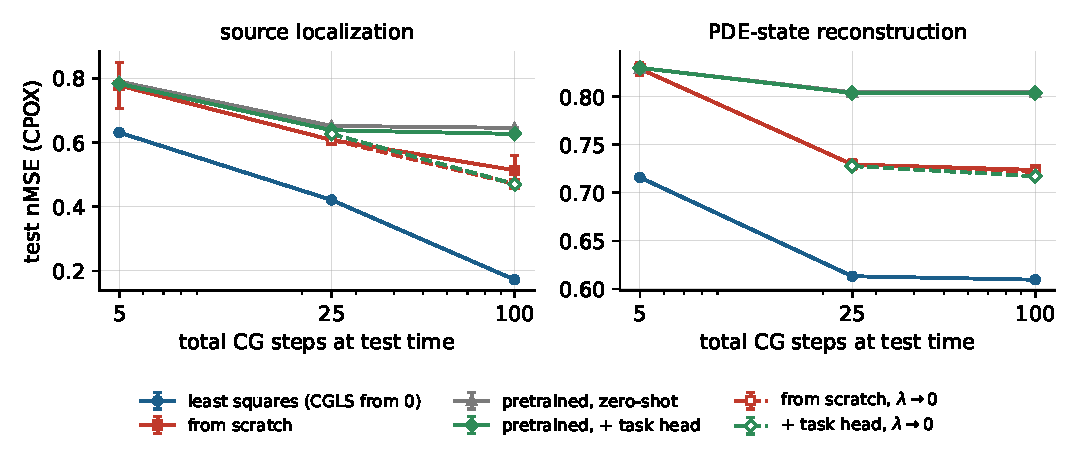
\includegraphics[width=\linewidth]{figures/solver_budget.pdf}
\caption{Test nMSE against the total CG budget at test time on the two ill-conditioned operators (held-out-task
cells of experiment A; learned models: mean $\pm$ std over 3 seeds; dashed: the same checkpoints with
$\lambda_{\text{task}}$ overridden to $10^{-8}$). Plain CG keeps improving on the noise-free source-localization
problem; the learned models, which restart CG from the backbone output in every unrolled iteration, do not,
with or without the data-consistency weight.}
\label{fig:budget}
\end{figure}

\section{Implementation details and hyperparameters}
\label{app:impl}
\begin{itemize}\setlength{\itemsep}{1pt}
\item \textbf{Backbone.} \texttt{graphHyperResNet}: 32 layers, 32 channels, leapfrog (hyperbolic) residual
updates with GCN-normalised, row-normalised edge weights, no dropout. Layers are gradient-checkpointed when a
batch has more than 20k edges (memory only; outputs identical).
\item \textbf{Heads.} Per task one linear encoder $\mathbb{R}^{2} \to \mathbb{R}^{32}$ (measurement and the
observation indicator $A^{\top} A \mathbf{1}$) and one linear head $\mathbb{R}^{32} \to \mathbb{R}$. Node
features: seasonal $(\sin, \cos)$ of the week and an observed-node flag for CPOX; a constant and the flag in B
(the native features of the B datasets are lagged copies of the target and would leak it).
\item \textbf{Data consistency.} \texttt{--dc prox}: 5 CG steps on $(A^{\top}A + \lambda I)x = A^{\top}b + \lambda x_{\text{ref}}$
warm-started at $x_{\text{ref}}$, $\lambda_{\text{task}} = \exp(20\,\ell_{\text{task}})$ with $\ell$ learned
(initialised at $\lambda = 0.01$). Denoising: $x = (b + \mu x_{\text{ref}})/(1 + \mu)$, $\mu = \mathrm{softplus}(m)$ learned.
Five unrolled iterations (\texttt{--solveIter 5}, \texttt{--cglsIter 5}).
\item \textbf{Operators.} Denoising $\sigma = 0.25$; inpainting budget 6 observed nodes per snapshot (random);
sensor recovery 5 sensors grown by BFS from a random seed node; source localization $\hat A^{4}$ with
$\hat A$ the GCN-normalised adjacency with self loops; PDE $\exp(-20 L)$ with $L$ the symmetric normalised
Laplacian, applied in the eigenbasis (fixed coefficients $K = 1$, $r = 0$). Graphs are made undirected
before normalisation.
\item \textbf{Optimisation.} Adam (amsgrad, $\epsilon = 10^{-3}$), lr $10^{-3}$, weight decay $4 \cdot 10^{-6}$,
batch 4 snapshots, gradient-norm clipping 1.0; heads lr $10^{-4}$. Epoch budget 40 + 16 + 4; from-scratch
baselines 60. Checkpoint selection on validation nMSE of the tasks trained in that phase.
\item \textbf{Data.} CPOX: 520 weekly snapshots, 20 nodes, 102 directed edges; train = first 81\,\%,
validation = next 9\,\%, test = last 10\,\% (chronological). B: CPOX, PedalMe (34 snapshots, 15 nodes,
complete), MontevideoBus (743 snapshots, 675 nodes, 690 edges) as training sets with a 10\,\% chronological
validation tail each; WikiMaths (1068 nodes; 20\,\% of snapshots) and Windmill (319 nodes, complete; 5\,\%
of 17k snapshots) test-only. Held-out dataset = whole series. Batches never mix datasets.
\item \textbf{Classical baselines.} CG on the normal equations from zero;
$\lambda \in \{0\} \cup \{10^{k/2}: k = -12, \dots, 4\}$, CG steps $\in \{5, 25, 100\}$, selected per task and
regulariser by the mean validation nMSE (CPOX validation weeks in A; in B the first 5 validation batches, i.e.\
20 snapshots, of each training dataset). Selected values are printed in \texttt{results/run\_eval\_cpu.log}.
\item \textbf{Provenance of the B table.} The classical rows of Tables~\ref{tab:b} and \ref{tab:b_full} were
computed on CPU; the learned rows are those printed by the same evaluator at the end of the GPU run
(\texttt{results/run\_gpu\_CB.log}), because re-running the 30 checkpoints on the Windmill test set is slow on
a CPU. The two differ only in the noise draw of the denoising task (GPU generator in that run), which moves
nMSE in the third decimal; every other task's measurements are identical.
\end{itemize}

\section{Known failure cases}
\label{app:fail}
\begin{itemize}\setlength{\itemsep}{1pt}
\item \textbf{Ill-conditioned operators (A).} All learned models are worse than plain CGLS on
source localization and PDE reconstruction; the pretrained model is worse than from-scratch there, and no
test-time setting of the solver (Table~\ref{tab:abl_full}) changes the ranking against plain CG. The held-out
PDE model stays at the level of $x = b$ (0.80 vs.\ 0.82) until its untrained data-consistency weight is removed
(0.73; plain CG 0.61). Running the from-scratch PDE model for 10 instead of 5 unrolled
iterations at test time diverges on one seed ($0.92 \pm 0.29$).
\item \textbf{Denoising.} No learned model beats a tuned scalar shrinkage of the measurement (0.281); the
learned prior does not add to the closed-form data step on this signal.
\item \textbf{CPOX held out in B.} With only PedalMe and Montevideo as training graphs the model is worse than
least squares on four tasks and unstable across seeds (inpainting $0.81 \pm 0.16$, source localization
$0.80 \pm 0.23$).
\item \textbf{Montevideo held out in B.} On the sparse 675-node graph the model is behind the tuned classical
solvers on every task and above zero-fill on both mask tasks (1.02, 1.05): the prior, trained on CPOX and
PedalMe, adds energy where the measurement has none.
\item \textbf{Sensor recovery on complete graphs (B).} The tuned graph-Laplacian solver beats the learned prior
on PedalMe (0.58 vs.\ 0.60) and Windmill (0.83 vs.\ 0.91); the prior only wins inpainting there.
\item \textbf{Complete graphs.} PedalMe and Windmill have a two-eigenvalue Laplacian; source localization and
PDE reconstruction collapse to mean recovery and every method reports the same number.
\item \textbf{Preliminary runs (not reported).} Earlier runs selected checkpoints on the test split, let the
PDE coefficients train, trained with an observation flag that evaluation did not use, and loaded checkpoints
with a head-aliasing bug; all were fixed before the reported runs (engineering log in
\texttt{CHANGES\_SUMMARY.txt}). An earlier WikiMaths run diverged (nMSE $> 10^{3}$) because the directed
533-out-degree hub was normalised as undirected; graphs are now symmetrised first.
\end{itemize}

\section{Reproducibility and compute}
\label{app:repro}
Code: \url{https://github.com/yakovge/GraphInverseProblems}, branch \texttt{final}. \texttt{bash run\_gpu.sh}
trains experiments A, C (from-scratch) and B and writes both tables; the three evaluation scripts
(\texttt{src/plot\_fixed.py}, \texttt{src/plot\_2.py}, \texttt{src/ablate\_solver.py}) re-evaluate the released
checkpoints in \texttt{results/} and reproduce every number in this paper (the README lists the exact
commands); \texttt{paper/make\_tables.py} builds the tables from their CSV output.
Training: 45 runs (5 per experiment A, C, B $\times$ 3 seeds; 75 checkpoints, since A and B save a zero-shot
and a task-head checkpoint per run); A on an 8-core laptop CPU in 2\,h\,05\,min, C + B on one NVIDIA
GTX 1080\,Ti in 23\,h\,15\,min (torch 2.7.1 + cu126). Evaluation: CPU, under two hours
for all tables. No NaN, divergence or out-of-memory event occurred in the reported runs.

\end{document}
